\chapter{Results}
\label{cha:results}
In this chapter the identified models generated by the
\Autoref{alg:identification} are discussed. The models are obtained through the
execution of the identification algorithm using modified paths with different
values of $k$.

\section{Identified Model}
In this work, we assume that all
sequences of events that have length $n_0+1$ were observed, so 
$L_{OrigNI}^{\leq n_0}=\emptyset$ can be true. In order to observe these
sequences of events, the observation of the system must be made for a sufficiently
long time. Thus, an experiment was made in order to observe the fault-free
behaviour of the system. The experiment lasted for 2
hours, time in which was possible to assemble and store over 100 cubes. A time
lapse of part of the experiment can be seen in
\url{https://www.youtube.com/watch?v=ZtCCKJtA9pI}.

The acquisition of the \emph{IOvectors} started once the system was initialised, that means,
when the system was ready to begin the process, this correspond to place
\hyperlink{partialTable:p27}{$p_{27}$} in \Autoref{fig:petriInitialization}.
The collected data\footnote{Available at:
  \url{https://raw.githubusercontent.com/Accacio/docsTCC/master/data/2019-05-10/2019-05-10_1524.csv}}
of this experiment has 19751 entries using 65
variables, the inputs\slash outputs of the system and the auxiliary variables
\verb|ConcUP| and \verb|ConcDWN|, presented in \Autoref{sec:implementation}.

Once this data was collected, the paths were obtained from the \verb|.csv| using
the method shown in \Autoref{sec:modIdent} and the
result was startling. The total number of paths obtained was equal to
2. This result can be easily explained by the behaviour of the system. The
system is formed of different modules, and it presents a considerable concurrent behaviour. And since these modules are not necessarily
synchronised, it is very unlikely that all of the modules will return to their initial
state at the same time. As presented in the path acquisition method, in order to generate
a new path it is needed that the \emph{IOvector} be the same as the initial
vector. Thus, the concurrent behaviour of the system results in a few very long paths. 


As expected, with a greater value of $k$, more states are identified. 
\Autoref{fig:statesIdentOriginal} shows the variation of the number of
states with respect to the value of $k$.
\begin{figure}[H]
  \centering
  \includegraphics[width=0.5\textwidth]{results/all/states.pdf}
  \caption{Number of states of identified model for different values of $k$.}
    \label{fig:statesIdentOriginal}
\end{figure}

The number of identified states for all values of $k$ is greater than $1000$. As
state transition diagrams representing the identified model would be almost
incomprehensible, a tool was developed to generate the \ffunction{} function of
the identified model. This tool is presented in \Autoref{sec:daoct}.

The \ffunction{} function generated using the original \verb|.csv| file
for $k=1$ and $k=2$
can be seen in  
\url{https://raw.githubusercontent.com/Accacio/docsTCC/master/figures/results/all/flistk1.tex}
% \Autoref{sec:originalKone}
and
\url{https://raw.githubusercontent.com/Accacio/docsTCC/master/figures/results/all/flistk2.tex}
% \Autoref{sec:originalKtwo}
respectively.

A comparison between the exceeding language generated by the
identified model using the \DAOCT{} model and the \NDAAO{} model, proposed by
\cite{klein2005fault}, can be made. This comparison shows that even for a considerable
large system with more than 60 inputs\slash outputs, the \DAOCT{} is more
tailored for fault detection. The cardinality of the exceeding language of the
\DAOCT{} model is
inferior to that of a \NDAAO{} model of the same size (with a similar \ffunction{} function).

\Autoref{fig:daoctNdaaoOriginal} shows the comparison between both models using 2 values of $k$.
In this case, considering $k=1$ and $n=12$ the
exceeding language of \NDAAO{} is $1018$ and for \DAOCT{} it is $923$. For $k=2$, both are $0$ for $n\leq12$. This mean in this case, with very
long paths, both have a similar behaviour, but \DAOCT{} still have a smaller exceeding language.
\begin{figure}[H]
  \centering
  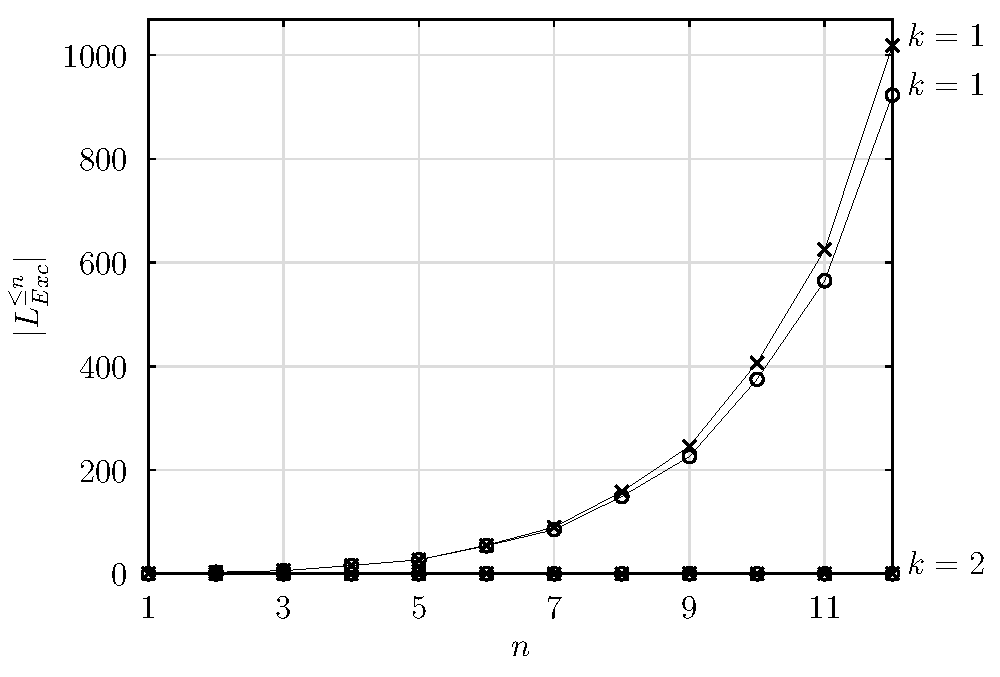
\includegraphics[width=0.5\textwidth]{results/all/exceedingLanguage-daoct-ndaao_k1-2_n12.pdf}
  \caption{Comparison between the cardinality of the exceeding language generated by the DAOCT (o) and
NDAAO ($\times$) models, for $k=1$ and $k=2$.}
    \label{fig:daoctNdaaoOriginal}
\end{figure}

% \subsection{best}
Since using the path acquisition method on the original \verb|.csv| file could obtain only 2 paths, an
experiment was made in order to increase the number of paths and see how
different the generated model would be.

The file was processed by a tool, where all vectors
were sorted by the number of duplicates in the file. The vector with most
duplicates was elected to be the new initial vector, consequently the initial
state of the new model.

A new \verb|.csv| file was created from the original one. The file was created by
discarding all vectors from the beginning of the file up to the
first appearance of the new initial vector. Then, this new initial vector is used
for the path acquisition method.

Instead of the original 19751 entries, the new
file 
had 19427 entries, since, some entries were discarded from the original. The difference in number of entries was reflected in the number of
generated states.

Using the path acquisition method in the modified file resulted in 80 paths, 40 times the
number of paths of the original.  

\Autoref{fig:statesIdentBest}
shows the variation of number of states with respect of the values of $k$.
% This
% figure can be used to see the relation
% between the change in the number of entries on the \verb|.csv| file and the
% number of generated states.
\begin{figure}[H]
  \centering
  \includegraphics[width=0.5\textwidth]{results/all/best/states.pdf}
  \caption{Number of states of identified model for different values of $k$.}
    \label{fig:statesIdentBest}
\end{figure}
Although both \Autoref{fig:statesIdentOriginal,fig:statesIdentBest} have the same order of magnitude for
each $k$, the number of states diverges. Putting the values in a vector can be
useful to
compare them. While for the original file the corresponding vector is
$\colvec{1321& 2166& 2962& 3744& 4508& 5235& 5939}$, for the modified is 
$\colvec{1294& 2127& 2904& 3663& 4395& 5088& 5746}$.
The difference in the number of identified states can be caused by the difference in the number of entries
in the \verb|.csv| files.

 The list of \ffunction{} functions generated using the modified \verb|.csv| file
for $k=1$ and \mbox{$k=2$}
can be seen in  
\url{https://raw.githubusercontent.com/Accacio/docsTCC/master/figures/results/all/best/flistk1.tex}
% \Autoref{sec:bestKone}
and
\url{https://raw.githubusercontent.com/Accacio/docsTCC/master/figures/results/all/best/flistk2.tex}
% \Autoref{sec:bestKtwo}
respectively.

The same comparison between the \DAOCT{} and \NDAAO{} models from
\Autoref{fig:daoctNdaaoOriginal} is shown in \Crefrange{fig:daoctNdaaoBestkone}{fig:daoctNdaaoBestkthree}.

In this second case we can see that the difference between the language of the \DAOCT{} and
\NDAAO{} models is more substantial. For example, for $k=1$ and $n=12$ the
exceeding language of \NDAAO{} is $465332$ and for \DAOCT{} it is $24866$. For
$k=2$ and $n=12$, it is $1943$ and $3$, for \NDAAO{} and \DAOCT{} respectively. And
if we take $k=3$ and $n=12$, it is $712$ for \NDAAO{} and $0$ \DAOCT{}. With
smaller and more numerous paths, we can see more clearly the difference between the
exceeding language of the models. For instance if we want to detect correctly
the failures of the system for sequences of length equal to or smaller
than $12$, using the \DAOCT{} model it is needed only to use a $k=3$ while for the
\NDAAO{} it is needed to use a $k$ greater than 7. For $k=7$ and $n=12$ the
exceeding language of \NDAAO{} is still equal to $47$. Showing that \NDAAO{} is more
computationally expensive for the identification of a system.

\begin{figure}[H]
  % \centering
  \begin{subfigure}[H]{0.5\textwidth}
    \centering
    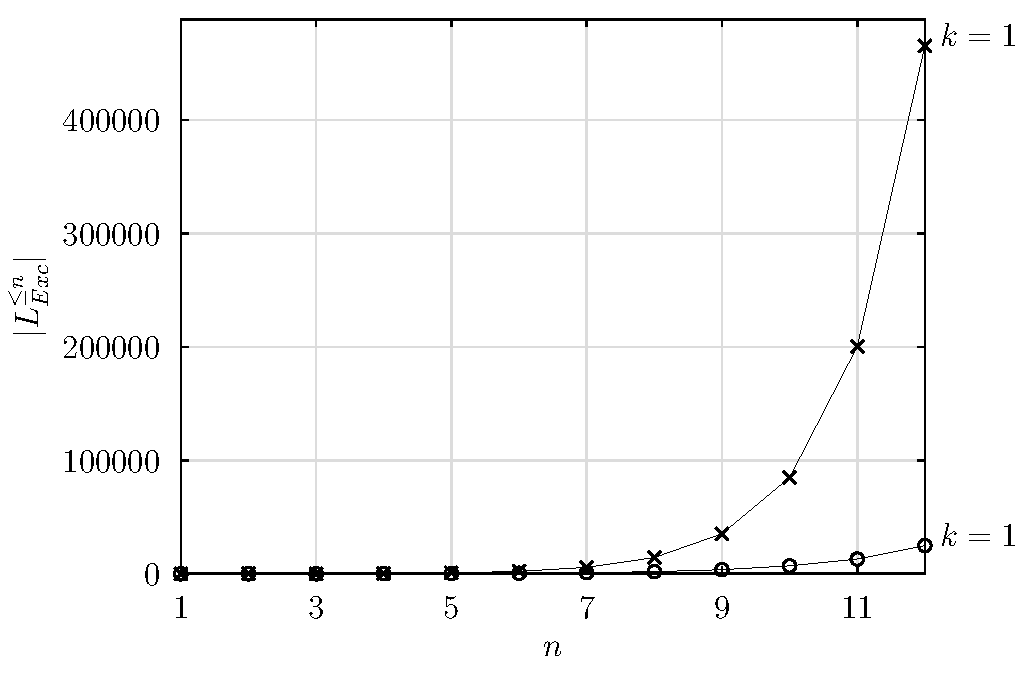
\includegraphics[width=\textwidth]{results/all/best/exceedingLanguage-daoct-ndaao_k1_n12.pdf}
    \caption{$k=1$}
    \label{fig:daoctNdaaoBestkone}
  \end{subfigure}
  ~
  \begin{subfigure}[h]{0.5\textwidth}
    \centering
    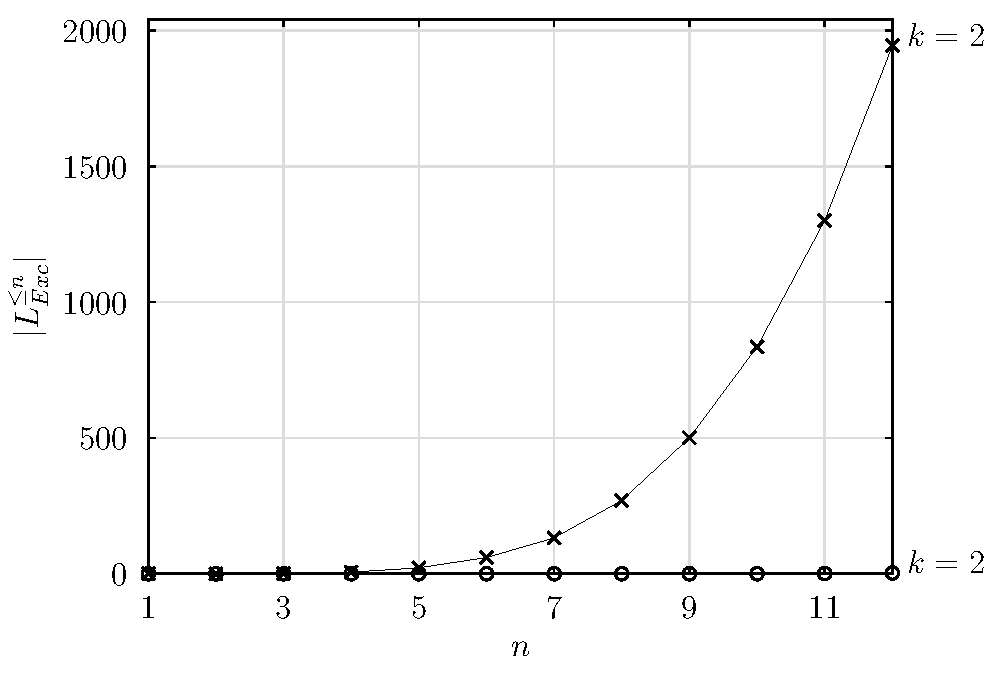
\includegraphics[width=\textwidth]{results/all/best/exceedingLanguage-daoct-ndaao_k2_n12.pdf}
    \caption{$k=2$}
    \label{fig:daoctNdaaoBestktwo}
  \end{subfigure}
  % \begin{center}
  \begin{subfigure}[h]{0.5\textwidth}
    \centering
    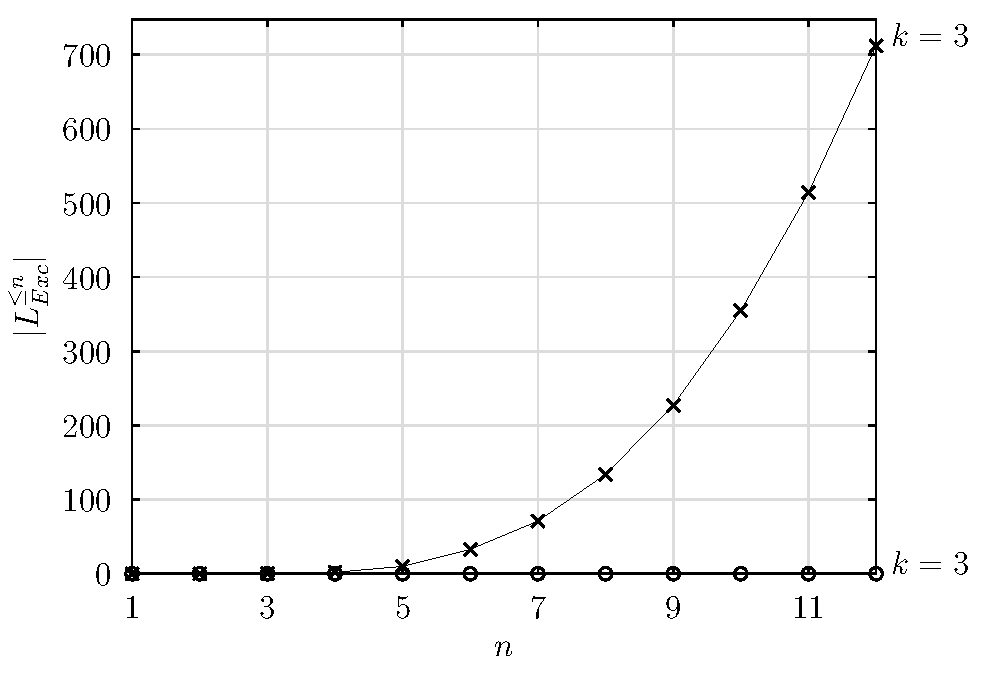
\includegraphics[width=\textwidth]{results/all/best/exceedingLanguage-daoct-ndaao_k3_n12.pdf}
    \caption{$k=3$}
    \label{fig:daoctNdaaoBestkthree}
  \end{subfigure}
  \begin{subfigure}[h]{0.5\textwidth}
    \centering
    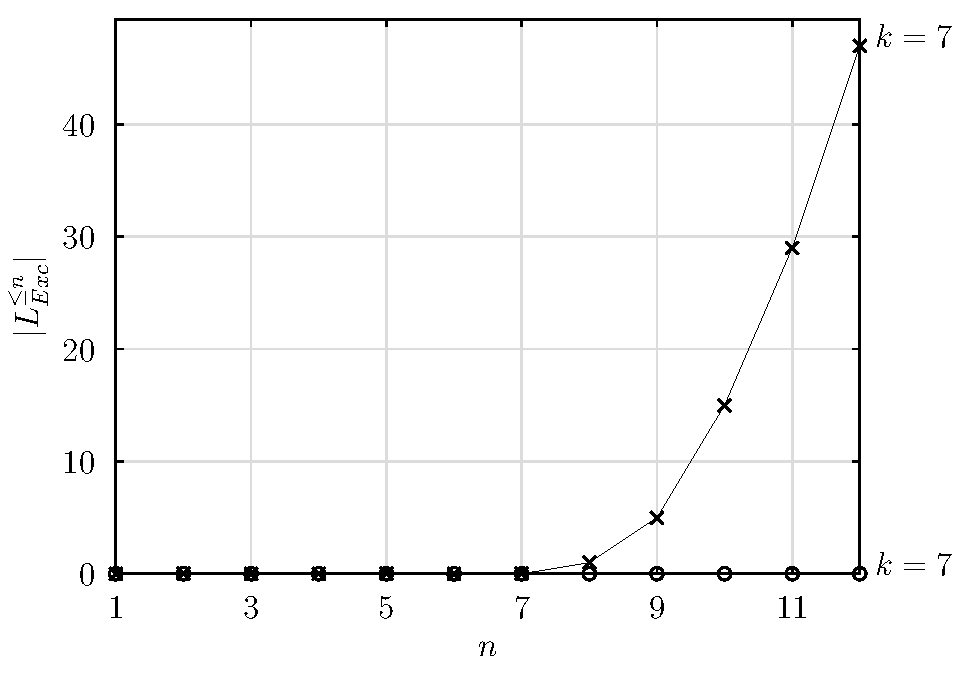
\includegraphics[width=\textwidth]{results/all/best/exceedingLanguage-daoct-ndaao_k7_n12.pdf}
    \caption{$k=7$}
    \label{fig:daoctNdaaoBestkseven}
  \end{subfigure}
    % \end{center}
  \caption{Comparison between the cardinality of the exceeding language generated by the DAOCT (o) and
NDAAO ($\times$) models.}
\end{figure}
Although the modified \verb|.csv| generates more paths and shows a more
considerable difference in the exceeding language generated by both models, it
does not mean that the model identified from the modified \verb|.csv| represents better the
system than the model identified from the original \verb|.csv|.
The choice of the first vector of acquisition can affect directly the identified
model and how it represents the system. The choice of the first vector and how
it can influence the modelling is discussed in the
next section.
\newpage
\section{About the choice of the first vector}
Let us consider the following system as an example : 
\begin{example}[Conveyor Belt with 3 sensors]~\\
  \label{ex:conveyor}
 This simple system consists in a conveyor belt with three sensors $S_1$, $S_2$ and
 $S_3$. A scheme of the conveyor and its sensors can be seen in
 \Autoref{fig:schemeExConveyor}. The conveyor belt is used to transport boxes, from
 the left to the right. The boxes are placed one at a time, so only a box can be
 over the conveyor. Once the box is over
 the conveyor and begin to be transported, it activates and deactivates $S_1$,
 then activates and deactivates $S_2$ and
 finally activates and deactivates $S_3$. After $S_3$ is deactivated and the box
 falls from the conveyor belt, another
 box is placed over the
 belt restarting the cycle. Since only a box is placed over the belt,
 it is impossible for 2 sensors to be activated at the same time.  As the belt is always turned on, this system
 only has outputs (inputs to the controller). The outputs of the system are the signals of the three sensors $S_1$, $S_2$ and
 $S_3$.
\end{example}
\begin{figure}[H]
  \centering
  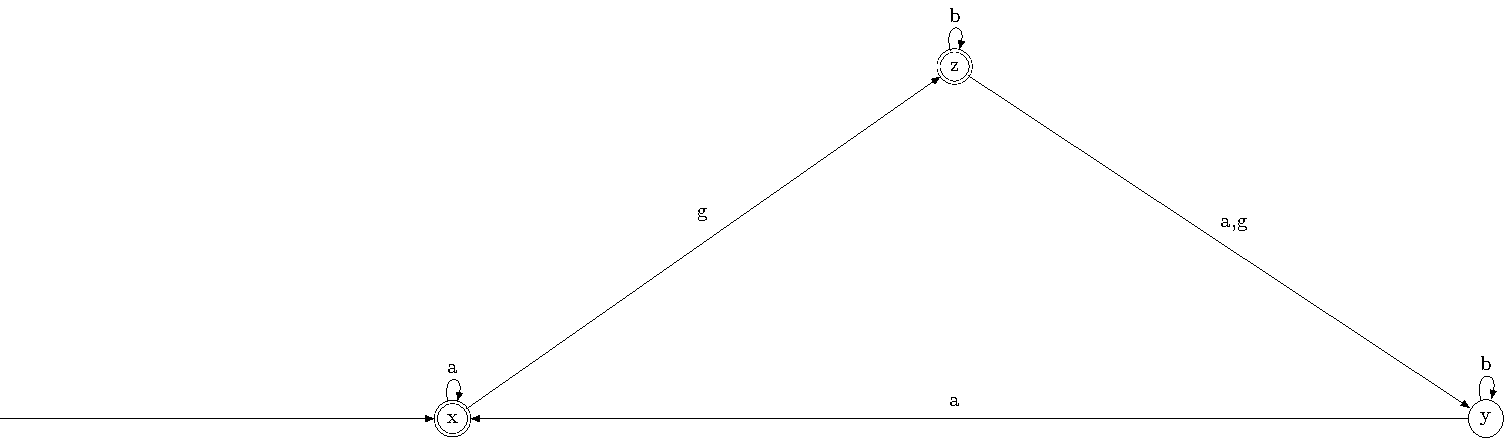
\includegraphics{results/example/example}
  \caption{Scheme of the example \ref{ex:conveyor}.}
    \label{fig:schemeExConveyor}
\end{figure}
If we make the data acquisition of this system and compose a vector with the
values of $S_1$, $S_2$ and $S_3$, we will have the following repeating motif:
\begin{align}
  \label{motif}
\colvec{0\\0\\0}\colvec{1\\0\\0}\colvec{0\\0\\0}\colvec{0\\1\\0}\colvec{0\\0\\0}\colvec{0\\0\\1}
\end{align}
This pattern will be repeated multiple times on the \verb|.csv| file forming
cycles, and since it forms cycles the pattern can be rewritten in how many ways as
it has vertices, in this case it can be written in 6 ways. To reduce the
complexity of the analysis we will only discuss 2 ways of writing it, the first
one shown in Equation
\ref{motif} and the second shown in Equation \ref{motifMod}. So, we can define two datasets of acquisition,
one beginning with $\colvec{0&0&0}^T$ and other with $\colvec{1&0&0}^T$.
\begin{align}
  \label{motifMod}
\colvec{1\\0\\0}\colvec{0\\0\\0}\colvec{0\\1\\0}\colvec{0\\0\\0}\colvec{0\\0\\1}\colvec{0\\0\\0}
\end{align}
If we take the first dataset, the one beginning with $\colvec{0&0&0}^T$, use the
path acquisition method and then
execute the identification algorithm, the identified model for $k=1$ can be
seen in \Autoref{fig:exampleCol000k1}. 
\begin{figure}[H]
  \centering
 \includegraphics{results/example/examplek1NoArrows}
  \caption{Identified model using $\colvec{0&0&0}^T$ as initial state, $k=1$.}
    \label{fig:exampleCol000k1}
\end{figure}
From the arcs of the state transition diagram, we can distinguish three paths. Since
$\colvec{0&0&0}^T$ is considered the first vector and it repeats thrice
throughout the motif, every time it is repeated another path is created.

But if we take the second dataset, the one beginning with $\colvec{1&0&0}^T$ the identified model for $k=1$ can be
seen in \Autoref{fig:exampleCol100k1}. 
\begin{figure}[H]
  \centering
  \includegraphics{results/example/example1k1NoArrows}
  \caption{Identified model using $\colvec{1&0&0}^T$ as initial state, $k=1$.}
    \label{fig:exampleCol100k1}
\end{figure}
Differently, only one path is created this time. In this figure we can see the
the vector $\colvec{0&0&0}^T$ represented as the state
$x_1$ in this state transition diagram. All other states have arcs coming
from or going to it. Using a greater value of $k$, $k=2$, for instance, we can have a
better vision of this unique path, see \Autoref{fig:exampleCol100k2}.
\begin{figure}[H]
  \centering
  \includegraphics[width=\textwidth]{results/example/example1k2NoArrows}
  \caption{Identified model using $\colvec{1&0&0}^T$ as initial state, $k=2$.}
    \label{fig:exampleCol100k2}
  \end{figure}

  In the first case, using $\colvec{0&0&0}^T$ as the initial vector, two more
  paths were created when comparing with the second case, where
  $\colvec{1&0&0}^T$ is used as the initial state. At a first glance it could
  seem that these 2 additional paths increase the reliability of the identified model,
  but actually, it does not. If we consider the allowed
  sequences on this first case, we can see that the events $\uparrow 2$ and
  $\uparrow 3$ are allowed even before the event $\uparrow 1$ is triggered,
  which is not part of the normal functioning of the system, described in
  example \Autoref{ex:conveyor}.

  So, even with only one path, the second case, using $\colvec{1&0&0}^T$ as
  initial state, represents better the system, since $\uparrow 3$ can only happen
  after the $\downarrow 1\uparrow 2\downarrow 2$ sequence, as described in
  example \Autoref{ex:conveyor}. It is important to notice that this
  representation is not perfect, but represents better the system than the model
  using $\colvec{0&0&0}^T$ as initial state.

  From this example we can verify that the choice of the first vector plays a very important part on
  the
  path acquisition method and consequently on the identified
  model.
  \begin{observation}
  An important remark to make is to show that we could only tell
  which identified system was more trustworthy because of the description of
  example \ref{ex:conveyor}. But once we have some information about the system,
  the system ceases to be a black box, and it becomes a grey box. 
\end{observation}

This remark shows that the success of the \DAOCT{} model is very dependent on a good
choice of the initial vector, and consequently the initial state of the
system. A question remains to be answered: how can we be sure if the
initial state was well chosen if we do not have any information about the system's original behaviour?
Maybe the root of this problem resides on the fact that input\slash output vectors
are used to extract the paths and to create the events. An approach that could
fix the problem would be
making it the other way around. First developing an identification model that uses purely
the observation of the events. The events once observed are used to
extract the paths, and consequently to identify the system.
%%% Local Variables:
%%% mode: latex
%%% TeX-master: "../monografia"
%%% End:
